\documentclass[12pt]{amsart}

    \addtolength{\hoffset}{-2.25cm}
    \addtolength{\textwidth}{4.5cm}
    \addtolength{\voffset}{-2.5cm}
    \addtolength{\textheight}{5cm}
    \setlength{\parskip}{0pt}
    \setlength{\parindent}{15pt}
    
    \usepackage{amsthm}
    \usepackage{amsmath}
    \usepackage{amssymb}
    \usepackage[utf8]{inputenc}
    \usepackage[colorlinks = true, linkcolor = black, citecolor = black, final]{hyperref}
    
    \usepackage{graphicx}
    \usepackage{multicol}
    \usepackage{ marvosym }
    \usepackage{wasysym}
    \usepackage{tikz}
    \usetikzlibrary{patterns}
    
    \newcommand{\ds}{\displaystyle}
    \DeclareMathOperator{\sech}{sech}
    
    
    \setlength{\parindent}{0in}
    
    \pagestyle{empty}
    
    \begin{document}
    
    \thispagestyle{empty}
    
    {\scshape Nacchofer31} \hfill {\scshape \large Apuntes TSR Bloque 2} \hfill {\scshape Tema \#4}
     
    \hrule
    
    \medskip
    
    \textbf{- Aplicación distribuida}: Colección de 
    componentes heterogéneos dispersos sobre una red de 
    computadores para realizar una función determinada.
    
    
    \begin{itemize}
    
    \item  Nodos heterogéneos autónomos que cooperan y presentan dependencias entre ellos, con requisitos para su ejecución y seguridad (privacidad, autenticación,...).
    
    \item  Objetivo: Proporcionar servicio a sus usuarios, para ello sus componentes necesitan ser instalados en varios ordenadores.
    
    \end{itemize}
    
    \textbf{- El despliegue} contiene todas las tareas de la gestión del ciclo de vida de una aplicación 
    informática que suceden tras su desarrollo, presentados en el proceso de despliegue de un servicio:
       
    
    \begin{itemize}
    
    \item  Instalación y activación de programas (Resolver 
    las dependencias del 
    software y entre los agentes, configurar software, establecer orden en que arrancan los componentes,...).
    
    \item  Desactivación, detener el sistema de forma ordenada.
    
    \item  Actualización, reemplazar componentes (ej. nueva versión). 
    
    \item  Adaptación (sin detener el servicio) tras un fallo o recuperación de un agente, cambios en los agentes, escalado.
    
    \end{itemize}
    
    \textbf{- Programas + Despliegue = Servicios} Como resultado, se obtienen componentes de la 
    aplicación, que se despliegan para llegar a ser un servicio.
    
    \smallskip
    
    \textbf{- Acuerdos de nivel de servicio (SLA)} pueden ser establecidos en el área de los servicios distribuidos entre el proveedor de servicios y sus clientes.
    
    \begin{itemize}
    
    \item  Funcionalidad facilitada por el proveedor se ajusta a las necesidades y requsitos de los clientes.
    
    \item  Rendimiento suele depender de la carga. Clientes solicitan nivel mínimo de rendimiento. Proveedor solicita a los clientes que no excedan cierto nivel máximo de carga.
    
    \item  Disponibilidad: Proveedor garantiza que el servicio estará disponible cuando los clientes lo necesiten. El nivel de disponibilidad (en porcentaje de tiempo que el servicio estará accesible para responder a  solicitud) deberá establecerse en el SLA.
    
    \end{itemize}
    
    \textbf{- Tipos de servicio} se pueden encontrar dos tipos:
    \begin{itemize}
    
    \item  Efímeros, servicios de sesiones breves e interactivas de uso en ordenadores personales, por un solo usuario. Ej: procesador de textos, navegadores web, intérprete de órdenes...
    
    \item  Persistentes, sercicios siempre disponibles, usados concurrentemente por multitud de usuarios con conexiones remotas. Ej: banca, administración y comercio electrónicos,...
    \end{itemize}
    
    \textbf{- Automatización del despliegue}, para despliegues de gran escala. \begin{itemize}
    
    \item  Cada componente de la aplicación distribuida tiene su propio BLOB de código, fichero que mantiene el programa a ejecutar por el componente y una plantilla de configuración. órdenes...
    
    \item  Configuración global de la aplicación. Mantiene un plan de interconexión entre componentes (lista de dependencias que deben resolverse, lista endpoints expuestos). Decide dónde colocar cada instancia. 
    \end{itemize}
    
    \textbf{- Configuración:} Uno de los pasos iniciales del despliegue es la generación del descriptor de despliegue.
    
    \begin{itemize}
    
    \item  Las plantillas de configuración de cada componente deben rellenarse tantas veces como instancias vaya a tener el componente.
    
    \item  La información para rellenar estas plantillas consiste en la resolución de dependencias.
    
    \item  Cada componente ejecuta cierto programa y ese programa exporta uno o más puntos de acceso y de dependencias que raramente podrán solucionarse en el proceso de compilación sino en el despliegue o la ejecución del programa (Resolución dinámica).
    
    \item No se requiere ningún cambio en la forma en que se escribe el código de las bibliotecas o el código de los programas que las utilicen (Transparencia para el programador).
    
    \end{itemize}
    
    
    \vfill
    
    \newpage
    
    {\bf - Los Contenedores} son herramientas que mantienen a otros componentes software, proporcionando un entorno aislado (protegido) y pueden establecer una correspondencia entre sus puntos de acceso y los del ordenador anfitrión.
    
    \begin{itemize}
    
    \item Gestionan las etapas del ciclo de vida de los componentes instalados en ellos, generando estos eventos del ciclo de vida:
    
    \subitem - Creación: órdenes para construir una imagen válida del componente.
    
    \subitem - Registro (initiate): registro de la imagen en el sistema de contenedores.
    
    \subitem - Inicio (start): Inicia la ejecución del componente en algún contenedor.
    
    \subitem - Parada: Ejecución del componente, después podrá ser reaunudado o finalizado.
    
    \subitem - Reconfiguración: Modifica el contenido de la imagen modificando sus módulos.
    
    \subitem - Destrucción: Elimina la imagen del componente del sistema de contenedores.
    
    \item  Aprovisionamiento (provisioning) consiste en la tarea de reservar la infraestructura necesaria para que una aplicación distribuida pueda funcionar.
    
    \subitem  Reservar recursos para cada instancia de componente (procesador + memoria + almacenamiento) y para la intercomunicación entre componentes.
    
    \subitem  La infraestructura suele concretarse en un pool de máquinas virtuales interconectadas, el componente y sus requisitos se implementan y ejecutan sobre una máquina virtual.
    
    \item  Inconveniente: Son menos flexibles que las máquinas virtuales, ya que el software de la instancia ha de ser compatible con el anfitrión y el aislamiento entre contenedores no es perfecta y esto puede provocar interferencias y problemas de seguridad.
    
    \item  Ventajas: Utiliza mucho menos recursos, consumen aproximadamente entre 10 y 100 veces menos recursos (reduce espacio). Si la parte inmutable se encuentra "precargada", se ahorra (90\%) para iniciar cada instancia (reduce tiempo). Mayor facilidad de despliegue (fichero de configuración). Aplicable en casi todos los escenarios.
    
    
    \end{itemize}
    
    {\bf - La inyección de dependencias} permite que el componente C sólo necesitará conocer la interfaz del servidor S para interactuar con él, que será implementada por una clase de proxy. El proxy P usado para interactuar con S es inyectado en C cuando se realiza el despliegue.
    \begin{itemize}
    
    \item  El proxy P usado para interactuar con S es inyectado en C cuando se realiza el despliegue.
    
    \item  Si el punto de acceso a S cambiara, el programa C no necesitará ser modificado, solo necesitaría una nueva versión del proxy P.
    
    \end{itemize}
    
    {\bf - Despliegue en la nube: IaaS}, en este modelo de despliegue:
    
    \begin{itemize}
    
    \item  La unidad a utilizar es la máquina virtual (MV). El proveedor ofrece un conjunto de tipos, según el tamaño y su capacidad de cómputo.
    
    \item  Presenta limitaciones, ya que este es demasiado primitivo:
    
    \subitem - No existen reglas que automaticen las decisiones de escalado de los componentes desplegados (bajo nivel).
    
    \subitem - No facilita herramientas para monitorizar el tráfico de red y seleccionar la ubicación de la MV.
    
    \subitem - Presenta un modelo de fallo insuficiente, los nodos de fallo no son realmente independientes y presenta una ayuda limitada frente a la recuperación.
    
    \end{itemize}
    
    {\bf - Despliegue en la nube: PaaS}, presenta mejoras de automatización del despliegue frente a las del modelo (IaaS):
    
    \begin{itemize}
    
    \item  Tiene como objetivo automatizar las tareas del ciclo de vida de los servicio.
    
    \item  La clave es el uso del SLA: El proveedor PaaS rellena un plan de despliegue y establece las reglas de escalabilidad a utilizar para obtener una adaptabilidad óptima, además de gestionar las actualizaciones del software de servicio respetando el SLA. 
    
    \item  Desafortunadamente los proveedores PaaS actuales no han alcanzado estos objetivos.
    La automatización es limitada, no se automatizan las decisiones de escalado con precisión, ya que no hay gestión del SLA ni actualizaciones.
    
    \end{itemize}
    
    {\bf - Docker}, ofrece una API para ejecutar procesos de forma aislada. 
    
    \begin{itemize}
    
    \item  Toma como base para construir una PaaS.
    
    \item  Soporta control de versiones (Git).
    
    \item  Define un sistema de ficheros de solo lectura para compartición entre contenedores.
    
    \item  Permite cooperación en el desarrollo mediante depósitos públicos.
    
    \item Presenta los siguientes componentes:
    
    \subitem - Imágenes (componente contructor): plantillas de solo lectura sobre las que se instancian contenedores.
    
    \$ docker build -t nombre\_imagen: Contruir una imagen a partir de un Dockerfile.
    
    \$ docker images: Muestra las imágenes creadas.
    
    \subitem - Depósito (componente distribuidor): depósito común para poder subir y compartir imágenes.
    
    \subitem - Contenedores (componente ejecutor): se crean a partir de imágenes, contienen todo lo necesario para ejecutarse.
    
    \$ docker run nombre\_imagen -i -t nombre\_contenedor: Tomar una imagen base y crear el contenedor.
    
    \$ docker commit id\_contenedor nueva\_imagen: Guardar ese estado como una nueva imagen.
    
    \end{itemize}
    
    {\bf - Órdenes en el archivo Dockerfile} 
    \begin{itemize}
    
    \item  FROM imageBase, primera instrucción (primera línea)
    
    \item MANITAINER nombre\_autor, establece el autor de la imagen.
    
    \item  ADD origen destino, Copia archivos de un lugar a otro. Origen suele ser un URL o un directorio (se copia el contenido) o un archivo accesible en el contexto de esa ejecución. Destino es una ruta en el contenedor.
    
    \item COPY origen destino, igual que ADD, pero no expande los ficheros comprimidos.
    
    \item RUN orden, ejecuta una orden (shell o exec), añadiendo un nuevo nivel sobre la imagen resultante.
    
    \item EXPOSE puerto, indica el puerto en el que el contenedor atenderá (listen) peticiones.
    
    \item  WORKDIR path, indica el directorio de trabajo para las órdenes RUN, CMD, ENTRYPOINT.
    
    \item USER uid, establece el UID bajo el que se ejecutará la imagen.
    
    \item ENV variable valor, asigna valores a las variables de entorno accesibles por los programas dentro del contenedor.
    
    \item VOLUME ruta\_contenedor, acceso del contenedor a un dir. del anfitrión, requiere run.
    
    \item CMD orden arg1 arg2 ..., proporciona los valores por defecto en la ejecución del contenedor.
    
    \item ENTRYPOINT orden arg1 arg2 ..., ejecuta dicha orden al crear el contenedor (terminal al finalizar la orden).
    
    
    IMPORTANTE: Sólo debería haber como máximo una orden CMD o ENTRYPOINT (si hay más, ejecuta la última).
    
    \end{itemize}
    
    {\bf - Múltiples componentes en distintos nodos} Docker admite enlaces entre contenedores de forma automatizada mediante docker-compose:
    
    \begin{itemize}
    
    \item Docker Compose, aplicación para definir y ejecutar aplicaciones ubicadas en varios contenedores Docker, limitado a contenedores de un único nodo, pero puede completarse con otro software de orquertación para controlar un cluster.
    
    Se requieren de tres pasos para el despliegue:
    
    \subitem 1. Definir el entorno de la aplicación con un Dockerfile.
    
    \subitem 2. Definir los  servicios de la aplicación en un archivo docker-compose.yml para que puedan ejecutarse conjuntamente.
    
    \subitem 3. Ejecutar  docker-compose  up,  con  lo que  Compose  iniciará  y ejecutará  la  aplicación completa.
    
    Las ordenes más significativas de docker compose son:
    
    \subitem - build: (re-)construye un servicio.
    
    \subitem - kill: detiene un contenedor.
    
    \subitem - start, stop, restart: inicia, detiene, reinicia un servicio.
    
    \subitem - rm: elimina un contenedor detenido.
    
    \subitem - run: ejecuta una orden en un servicio.
    
    \subitem - scale: número de contenedores a ejecutar para un servicio.
    
    \subitem - up: build + start.
    
    \subitem - port: muestra el puerto asociado al servicio.
    
    \subitem - ps: lista los contenedores.
    
    \subitem - pull: sube una imagen.
    
    Ciclo típico de uso:
    
    \subitem \$ docker-compose up -d
    
    \subitem \$ docker-compose stop
    
    \subitem \$ docker-compose rm -f
    
    En la creación de un descriptor de despliegue docker-compose.yml siguiendo la sintaxis YAML, los parámetros principales son:
    
    \subitem - image: referencia local o remota a una imagen, por nombre o tag.
    
    \subitem - build: ruta a un directorio que contiene un DockerFile.
    
    \subitem - command: cambia la orden a ejecutar en el inicio.
    
    \subitem - links: enlace a contenedores de otro servicio.
    
    \subitem - external\_links: enlace a contenedores externos a compose.
    
    \subitem - ports: puertos expuestos (en comillas "").
    
    \subitem - expose: Ídem, pero accesible sólo a servicios enlazados (mediante links).
    
    \subitem - volumes: monta rutas como volúmenes.
    
    \item Kubernetes, orquestador de contenedores ajeno a Docker, para distribuir las instancias entre los distintos nodos. Presenta los siguientes elementos principales:
    
    \subitem - Cluster y nodo (máquinas físicas y virtuales respectivamente).
    
    \subitem - Pod, unidad más pequeña desplegable que contiene un conjunto de contenedores con namespace y volúmenes compartidos.
    
    \subitem - Controladores de replicación, se encarga del ciclo de vida de un conjunto de pods, asegura que esté ejecutándose la cantidad especificada de réplicas del pod. Escalando, recuperando y replicando pods.
    
    \subitem - Controlador de despliegue, actualizan la aplicación distribuida.
    
    \subitem - Servicio, define un conjunto de pods y la forma de acceder a ellos.
    
    \subitem - Secretos, gestión de credenciales de nuestras aplicaciones.
    
    \subitem - Volúmenes, gestión de la presistencia de contenedores.
    
    \end{itemize}
    
    
    \pagebreak
    
    {\scshape Nacchofer31} \hfill {\scshape \large Apuntes TSR Bloque 2} \hfill {\scshape Tema \#5}
    
    \hrule
    
    \medskip
    
    \textbf{- Fallo}, cuando algún componente del sistema es incapaz de comportarse de acuerdo con su especificación. Se deben distinguir entre defectos, errores y fallos:
    
    \begin{itemize}
        \item Defecto (fault), condición anómala, el componente es incapaz de reaccionar Ej: corte de alimentación eléctrica, error de diseño,...
        \item Error, manifestación de un defecto en un sistema, el estado de algún componente diferirá de su estado previsto.
        \item Fallo (failure), incapacidad para que un elemento desarrolle aquellas funciones para las que fue diseñado debido a errores en el propio elemento o en su entorno, que han sido causados por diferentes defectos.
    \end{itemize}
    
    Un fallo es el resultado de dos transiciones previas (defecto a error, error a fallo) y habría que intentar que ambas transiciones no llegasen a darse en el sistema.
    
    \textbf{- Transparencia de fallos}, todo sistema distribuido debe proporcionar trasparencia de fallos. 
    
    Los errores en algún componente, en caso de producirse, no deben ser percibidos por los usuarios. La solución es el proceso de replicación, la réplica con errores se aísla, se repara y se reincorpora, las demás ocultan esa situación.
    
    También se denomina "fault tolerance", un sistema tolera defectos cuando exhibe un comportamiento correcto en caso de que haya defectos. Un servicio tolera defectos si se diseña adecuadamente y, también toleran defectos todos aquellos servicios de los que dependa.
    
    \textbf{- Modelo de fallo}, los fallos pueden tener múltiples causas, depende de los defectos que haya y a qué componentes afecten, se pueden distinguir múltiples fallos. 
    
    Cuando se diseñan algoritmos distribuidos conviene asumir algún modelo de fallos, aunque ningún modelo puede reflejar con precisión todas las situaciones de fallo obteniendo una mayor abstracción, el middleware tendrá que aproximar estas situaciones que asuma el modelo.
    
    
    
    \begin{itemize}
    
    \item En la red, conviene evitar los fallos para una mejor conectividad entre los componentes ya que puede ocurrir que haya intervalos en los que la comunicación entre las diferentes redes no sea posible (partición de la red). Cuando se dé una partición un determinado subconjunto de nodos queda aislado del resto del sistema. Cuando se da una partición en la red, hay dos formas básicas de afrontarla:
    
    \subitem - Sistemas particionables, cada uno de los subgrupos aislados puede continuar con su trabajo. Los sistemas particionables necesitan algún protocolo de reconciliación para decidir de qué manera s reintegrarán todas las modificaciones aplicadas en cada réplica cuando los subgrupos recuperen su conectividad. 
    
    \subitem - Modelo de subgrupo primario (componente primario o partición primaria), solo se admite que continúe aquel subgrupo que tenga una mayoría de nodos que formaban en el sistema. Sin embargo, en una partición puede ocurrir que no haya ningún subgrupo mayoritario, en este caso deberían 
    
    \end{itemize}
    
    \textbf{- Replicación}, es el mecanismo para proporcionar transparencia de fallos y asegurar la disponibilidad de los servicios de un sistema distribuido, tienen las siguientes características:
    
    \begin{itemize}
        \item Las réplicas se ubican en ordenadores en una máquina distinta, que no dependan de una misma fuente de fallos. Ej: red eléctrica, SAI, red local,...
        \item Deben revisarse con cuidado las dependencias entre diferentes componentes. Cuando esa réplica falle, ese fallo debe aislarse para que el resto de los componentes que usen sus servicios no advierta esa situación.
        \item Las peticiones que haya en curso en la réplica defectuosa tendrán que ser reasignadas a una réplica correcta y ser reaunudadas de forma autónoma.
    \end{itemize}
    La replicación también mejora el rendimiento y la escalabilidad:
    
    \begin{itemize}
        \item Las operaciones de lectura que soólo quieran consultar el estado de un servicio (lectura) pueden ser ejecutadas por una sola réplica, con un excelente escalado lineal.
        \item Las operaciones de escritura deben ser aplicadas en todas las réplicas, requerirá de un esfuerzo para programarla y atenderla con retardos.
        
        - Si la operación es breve, puede ser ejecutada por todas las réplicas y habrá que propagar la petición a todas.
        
        - Si su ejecución es costosa pero solo modifica una pequeña parte del estado del servicio, ejecuta en una sola réplica, propagando las modificaciones al resto de réplicas.
        
        - El grado de divergencia determina el modelo de consistencia.
    \end{itemize}
    
    \textbf{- Modelo de replicación pasivo}, los clientes envían sus peticiones a la réplica primaria, una misma réplica para todos los clientes y todas las peticiones, que es la que ejecutará la operación.
    
    Al terminar, propagará las modificaciones a las réplicas secundarias y responde al cliente.
    
    \begin{itemize}
        \item Ventajas:
        
        - Mínima carga, la gestión de una operación recae en la réplica primaria. Las réplicas secundarias atienden las peticiones de solo lectura, así se reparte la carga.
        
        - Orden fácil de establecer, réplica primaria numera las difusiones y las envía a las secundarias.
        
        - Control de concurrencia local, el modelo admite ejecución concurrente por lo que no se necesitan algoritmos distribuidos.
        
        - Admite operaciones no deterministas, solo las ejecuta el primario y no se generarán inconsistencias.
    
    \item Inconvenientes:
    
    - Reconfiguración pesada cuando falle la réplica primaria, hay que seleccionar una secundaria y promoverlo a primero
    
    - No se soporta el modelo de fallos bizantino, como el cliente solo recibe una respuesta es incapaz de advertir si esta respuesta cuadra con lo esperado.
    \end{itemize}
    
    \textbf{- Modelo de replicación activo (máquina de estados)}, los clientes difunden sus peticiones a todas las réplicas del servidor. Cada réplica servidora ejecuta la operación, cuando una réplica termina, responde al cliente.
    
    \begin{itemize}
        \item Ventajas:
        
        - Reconfiguración trivial en caso de fallo, no se necesita realizar nada especial siempre y cuando quede alguna réplica.
        
        - Se soporta el modelo de fallos bizantinos, dados "f" fallos simultáneos, en el caso más favorable, se requiere 2f+1 réplicas, el cliente seleccionará la respuesta mayoritaria.
        \item Inconvenientes:
        
        - Si se necesita consistencia fuerte, las peticiones deben difundirse a todas las réplicas en orden total, esto requiere consenso, protocolo pesado.
        
        - No se toloeran operaciones no deterministas, ya que cada réplica debe ejecutar todas las operaciones y se obtienen un resutado diferente, provocaría inconsistencias.
        
        - Cuando interactúen servicios replicados bajo este modelo hay que filtrar las peticiones.
        
    \end{itemize}
    
    \begin{center}
    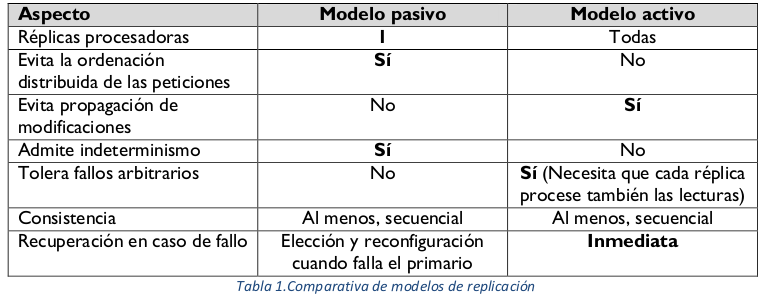
\includegraphics[width=13cm, height=6cm]{comparativa.png}  
    \end{center}
    
    \textbf{- Comparativa}, el modelo de replicación elegido depende de:
    
    \begin{itemize}
        \item El tiempo promedio de procesamiento para las peticiones:
        
        - El modelo pasivo es apropiado para procesamiento prolongado, pues solo afecta a la réplica primaria.
        
        - El modelo activo es apropiado para procesamiento breve.
        
        \item El tamaño de las modificaciones:
        
        - El modelo pasivo es apropiado para modificaciones pequeñas.
        
        - El modelo activo es apropiado para modificaciones grandes, ya que no necesita tranferirla a otras réplicas.
    \end{itemize}
    
    \textbf{- Consistencia}, cuando se replica información en múltiples nodos, un modelo de consistencia específica qué divergencias se admiten entre los valores de las réplicas de un mismo elemento. 
    
    \begin{itemize}
        \item Los clientes realizan la escritura inicialmente en un nodo que propaga posteriormente el resultado a las demás réplicas.
        \item La consistencia obtenida depende del retardo de esta propagación y las esperas que introduzca ese retardo en otros procesos.
        \item Algoritmo de consistencia: Para controlar esas acciones de escritura y las acciones de lectura, se utiliza un algoritmo de consistencia.
        
        - Algoritmo de consistencia rápido: Si este permite que tanto escrituras como lecturas retornen el control sin esperar a que se haya transmitido algún mensaje.
        
        - Algoritmo de consistencia lento: caso contrario.
        
        \item Modelos de consistencia:
        
        - Estricto (lento), propagación de las escrituras inmediata y mientras se ejecuta una escritura no se puede estar ejecutando ninguna otra escritura. Cada lectura siempre devuelve el valor de la última escritura realizada sobre la variable. Imposible de implantar.
        
        - Secuencial (lento), sigue una especificación informal, todos los procesos llegan a un acuerdo sobre el orden en que se han llegado a aplicar las escrituras sobre todas las variables que cuadra con el utilizado al escribir en cada proceso, pero cada uno puede avanzar "a su ritmo".
        
        - Caché (lento), requiere que las escrituras realizadas sobre una misma variable sean vistas en el mismo orden por todos los procesos. NO impone restricción a la hora de "mezclar" lo que se haya hecho sobre diferentes variables.
        
        - Procesador (lento), cuando se cumplen Caché y FIFO simultáneamente.
        
        - Causal (rápido), se respeta la relación de orden "happens before" por Lamport usada para definir los relojes lógicos. W(x) - R(x)a.
        
        - FIFO (rápido), requiere que las escrituras por un proceso sean leídas en orden de escritura por todos los demás procesos, pero no tiene restricción al "mezlcar" lo que han hecho diferentes escritores.
        
        \item Jerarquía de modelos, las flechas indican que el modelo es más estricto que el modelo destino, si se cumple origen, también destino:
        \begin{center}
    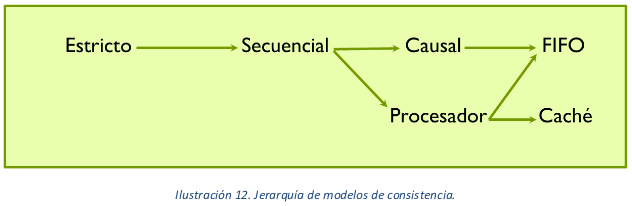
\includegraphics[width=8cm, height=3cm]{consistencias.png}
    \end{center}
    \end{itemize}
    
    \textbf{- Consistencia final}, es una condición que llegará a cumplirse cuando haya un intervalo suficientemente largo en el que no haya escrituras. Hay libertad completa para que las escrituras se realicen en cualquier réplica y se propaguen en el orden y con el retardo de cada escritor crea conveniente.
    
    \pagebreak
    
    {\scshape Nacchofer31} \hfill {\scshape \large Apuntes TSR Bloque 2} \hfill {\scshape Tema \#6}
    
    \hrule
    
    \medskip
    
    \textbf{- Los sistemas distribuidos son escalables} si puede manejar la adición de usuarios y recursos sin sufrir una pérdida apreciable de rendimiento o un incremento de su complejidad administrativa, sin generar ningún trastorno en la prestición de servicios.
    
    Esta definición incluye tres dimensiones en el estudio de la escalabilidad:
    
    \begin{itemize}
    
    \item  Escalabilidad de tamaño: Cuando el número de usuarios atendidos por el sistema llegue a crecer linealmente con el número de nodos.
    
    \item  Escalabilidad de distancia: Cuando tolera los problemas que comporta una mayor distancia entre sus nodos. Estos problemas son un mayor retardo de propagación, menor ancho de banda y una menor fiabilidad de transmisión.
    
    \item  Escalabilidad administrativa: Cuando el sistema admite que múltiples organizaciones colaboren en la administración de sus nodos.
    
    \end{itemize}
    
    Se pueden diferenciar dos clases de escalabilidad:
    
    \begin{itemize}
    \item Escalabilidad vertical ("Scale-up"): incrementar la capacidad de un nodo determinado reemplazando alguno de sus componentes hardware. Un caso extremo es la sustitución del nodo entero por otro con mejores prestaciones.
    
    \item Escalabilidad horizontal ("Scale-out"): añadir nodos al sistema, tradicionalmente se denomina escalabilidad de tamaño. 
    \end{itemize}
    
    \textbf{- El Teorema CAP}, enuncia el hecho de que en un sistema distribuido parcialmente sincrónico no se podrán cumplir simultáneamente estas tres propiedades (debería de sacrificar al menos una de ellas).
    
    \begin{itemize}
    \item Consistencia fuerte (C:"Consistency"), si se obliga a que todos los procesos correctos acepten operaciones de escritura y se pueden extender a otros modelos más relajados como el secuencial.
    
    \item Disponibilidad de los servicios (A:"Availability"), todo nodo correcto debe seguir aceptando y ejecutando peticiones (de lectura y escritura) independientemente del subgrupo de nodos al que pertenezca en caso de que divida la red.
    
    \item Tolerancia al particionado de la red (P:"Partition-tolerance"): La aplicación debe continuar su ejecución sin problemas a pesar de que haya particiones en la red.
    \end{itemize}
    
    \textbf{- Sacrificio de propiedades}, toda aplicación robusta debe renunciar a una de las tres propiedades, optando por estas tres opciones:
    
    \begin{itemize}
    \item Sacrificar P (tolerancia particiones), garantiza consistencia fuerte y disponibilidad total de los servicios. No se admitirá que la red se particione, sin embargo es  muy difícil de asegurar, solo se podría soportar en un despliegue local.
    
    \item Sacrificar A (disponibilidad), adoptada en los sistemas replicados, se pretende asegurar consistencia fuerte y tolerancia a las particiones.
    
    \subitem Cuando hay una partición se adoptará un modelo de partición primaria, solo el subgrupo mayoritario de nodos continuará (mantendrán consistencia fuerte), el reto parará (se perderá la disponibilidad en sus nodos, advirtiendo los clientes asociados de la situación).
    
    \item Sacrificar C (consistencia fuerte), garantiza la disponibilidad de todas los nodos correctos y la tolerancia del particionado de la red.
    
    \subitem Cuando hay una partición, se adoptará un modelo de sistema particionable. Al procesar escrituras en cada subgrupo, se perterá consistencia fuerte, los demás subrupos no pueden ver esas escrituras.
    Si se diseña con cuidado y las operaciones son conmutativas, se podrá obtener consistencia final.
    \end{itemize}
    
    La mejor opción es la de sacrificar la consistencia fuerte (es la que más ha tenido aceptación), ya que los servidores siempre deben estar disponibles, atendiendo a un número creciente de usuarios.
    
    \medskip
    
    \textbf{- Replicación de máquina de estados (Modelo pasivo)}, el rol primario es estático, todas las peticiones deben dirigirse al mismo primario, en todos los casos y para todos los clientes. Los modificadores de estado se propagan de forma síncrona, antes de enviar la respuesta al cliente.
    
    \textbf{- Replicación multi-master}, cada cliente envía su solicitud a una sola réplica: la máster. Cada petición puede ser enviada a una réplica máster diferente. El rol de máster se elige en cada solicitud y todas las réplicas deben seguir ambos roles, dependiendo de la elección del cliente. La propagación de los modificadores es perezosa, permitiendo una respuesta rápida a los clientes, así el tiempo de respuesta es más breve que el pasivo.
    
    Ventajas:
    
    \begin{itemize}
    \item Mínima sobrecarga, cada petición es procesada por una sola réplica, tanto para peticiones de solo lectura como modificación.
    
    \item Altamente escalable, no asume ningún mecanismo de control de concurrencia.
    
    \item Admite operaciones no deterministas, solo son ejecutadas por un máster, de forma que no surgirán inconsistencias entre réplicas por el servicio de una misma operación.
    \end{itemize}
    
    Inconvenientes:
    
    \begin{itemize}
    \item Las peticiones en curso pueden perderse cuando el máster falle, todos los pasos son asincrónicos, no hay garantías acerca de la finalización del proceso de la solicitud. 
    
    \item El modelo de fallos bizantinos no se soportaría, no hay forma de detectar cúando las respuestas de un máster son correctas.
    
    \item La consistencia de las réplicas es muy relajada, puede llegar a provocar divergencias.
    \end{itemize}
    
    \textbf{- Almacenes NoSQL}, Los SGBD relacionales, presenta múltiples limitaciones de escalabilidad, que se pueden resolver en la práctica mediante las siguientes vías:
    
    \begin{itemize}
    \item Simplificar el esquema de la base de datos, sustituyendo múltiples tablas con múltiples columnas por tablas clave/valor (índices simples).
    Implica el abandono del estándar SQL por un lenguaje de interrogación, para un procesamiento directo. El espacio ocupado por la base se reduce, que pueden mantenerse en memoria principal, se asegura la persistencia mediante replicación.
    
    \item Eliminando las transacciones, no se podrá asegurar una secuencia de sentencias en una misma transacción, la atomidicad será limitada a cada sentencia por separado.
    \end{itemize}
    
    \textbf{- Almacenes clave-valor}, ejemplos como Dynamo, Voldemort, Riak,...
    \begin{itemize}
        \item Solo se distingue dos campos: clave y valor, las búsquedas de información se realizan en base a clave.
        \item El atributo valor es el valor que el SGBD es incapaz de interpretar y es incapaz de buscar 'interrogar' o buscar por atributos no primarios.
    \end{itemize}
     \textbf{- Almacenes de documentos}, ejemplos como CouchDB, MongoDB, SimpleDB,...
     \begin{itemize}
         \item Los elementos que se guardan en la base de datos se denominan documentos, que tienen asociados un campo clave (identificador de documento) y una secuencia de atributos, que pueden ser a su vez otros objetos.
         
         \item El lenguaje de interrogación establece condiciones que deberían cumplir los documentos que se retornen como resultado de cada consulta, en forma de restricciones.
     \end{itemize}
     
    \textbf{- Almacenes de registros extensibles}, ejemplos como Bigtable, PNUTs, Cassandra,...
    
    \begin{itemize}
        \item Las bases se organizan en tablas, estas tablas tienen un número variable de columnas, a su verz, el conjunto de columnas puede organizarse en grupos de columnas.
        
        \item El particionado de documentos consiste en la posibilidad de añadir particionado vertical al horizontal
        
        \item El particionado mejora las prestaciones, reparte la responsabilidad entre múltiples nodos, obteniendo una mayor concurrencia.
    \end{itemize}
    
    \pagebreak
    
    \textbf{- Elasticidad}, es el grado en que un sistema es capaz de adaptarse a cambios en su carga suministrando y reciclando los recursos de una manera autónoma, cosiguiendo que en cada momento los recursos disponibles cubran la demanda existente con la mayor precisión posible.
    
    \begin{itemize}
        \item Debe ser escalable, debe ser capaz de atender cargas variables.
        
        \item Debe ser dinámico y adaptable, en función de la carga que haya en cada momento. 
        \item La adaptabilidad tiene que ser autónoma, el sistema tiene que ser capaz de decidir que cambios deben realizarse sin que intervenga ningún administrador.
    \end{itemize}
    
    Es una característica exigible a los sistemas cloud modernos, al ajustar el coste justo para el usuario y al administrar los recursos del proveedor. Para implantar un sistema elástico se necesitará:
    
    \begin{itemize}
        \item Un mecanismo de monitorización, que evalúe la carga soportada por cada uno de los recursos que formen el sistema y el rendimiento de los módulos que se hayan instalado en el sistema.
        
        \item Un sistema de actuación, para automatizar la reconfiguración de los servicios, en función del SLA establecido.
    \end{itemize}
    
    \textbf{- Contención y cuellos de botella}, el sistema distribuido está formado con múltiples componentes y existen dependencias entre ellos, para ello su diseño debe ser cuidadoso para evitar esta contención, las causas de la contención son:
    
    \begin{itemize}
        \item Uso de algoritmos centralizados para realizar tareas "pesadas".
        
        \item Uso de herramientas de sincronización, ya que habrá una sección crítica y su protección producirá bloqueos.
        
        \item Tráfico excesivo, una mala distribución de los recursos puede conducir a un incremento de las necesidades de comunicación remota.
    \end{itemize}
    
    Para evitar esta contención en función de su casa serían:
    
    \begin{itemize}
        \item Ante la centralización, gestionar las tareas pesadas y frecuentes usando algoritmos descentralizados, repartiendo la carga entre múltiples procesos.
        
        \item Ante el acceso a recursos compartidos, serializando los accesos y adoptando un paradigma de programación asincrónica, si no hay competición por el uso de los recursos gestionando la carga, resultando un sistema más eficiente.
        
        \item Por tráfico excesivo, replicar los recursos y mantenerlos consistentes, los accesos remotos se transforman en accesos locales.
    \end{itemize}
    
    \textbf{- Módulo cluster de NodeJS}, facilita la creación y gestión de un pool de trabajadores (procesos de Node) y el reparto equilibrado de la carga de servicio entre los procesos compartiendo todos los puertos asociados al sercicio que presten. Incluye un Worker que modela los procesos del cluster, son supervisados y creados por un proceso master.
    
    Dispone de eventos del objeto Cluster:
    \begin{itemize}
        \item fork, cuando se crea un nuevo worker.
        \item online, cuando se escribe un mensaje de un worker indicado que ha comenzado a ejecutarse.
        \item listening, cuando un worker ejecuta listen()
        \item disconnect, cuando el canal IPC de un worker se desconecta porque el worker termine, "exit" o eliminado "kill" o se desconecte "disconect"
        \item exit, cuando un worker muere.
    \end{itemize}
    \textbf{- MongoDB}, es un almacen de documentos escalable, una base de datos es un conjunto de colecciones (tablas). Cada colección es un conjunto de objetos estructurados, cada objeto tiene un identificador y múltiples atributos. Se utiliza particionado horizontal "sharding" de tipo replicación pasiva.
    Encontramos múltiples procesos:
    
    \begin{itemize}
        \item mongod, tiene un subconjunto de filas "shard", cada partición puede replicarse.
        \item mongos, actúan como interfaz con la aplicación cliente.
        \item Servidores de configuración, guarda metadatos de BD.
    \end{itemize}
    
    \end{document}